\documentclass[../main.tex]{subfiles}
\begin{document}
  
\section[Задача Коши для колебаний струны]{Задача Коши для уравнения колебаний струны. Формула Даламбера. Область зависимости решения от начальных данных. Существование и единственность классического решения. Корректность постановки задачи.}
% Затехал: Рязанов Андрей
\textbullet\ Задача: \quad $\begin{cases} u_{tt}-a^2u_{xx} = 0\\ \eval{u}_{t=0} = u_0(x)\\ \eval{u_t}_{t=0} = u_1(x)\end{cases}\quad -l<x<l$
\vspace{0.5em}

Что понимать под решением задачи?

\begin{definition} \textbf{\emph{Классическое решение}} -- функция класса $C^2$, которая в точках указанной области удовлетворяет уравнению и заданным соотношениям.
\end{definition}

\imaginarySubsection{Формула Даламбера}
\textbullet\ {\bf Характеристическое уравнение: } $(dx)^2 - a^2(dt)^2 = 0$

$\begin{cases} \xi = x+at \\ \eta = x-at \end{cases} \Leftarrow \begin{cases} x+at = C_1 \\ x-at = C_2 \end{cases}$

В новых координатах $\hat{u}_{\xi\eta}(\xi,\eta) = 0\ \Rightarrow \hat{u} = f(\xi) + g(\eta) $.

Возвращаясь обратно, получим $u(t,x) = f(x+at) + g(x-at)$.
\vspace{0.4em}

\textbullet\ Решим ЗК (поверхности нигде не касаются характеристик -- задача должна быть корректной):
\begin{equation*}
\begin{aligned}
&\eval{u}_{t=0} = f(x) + g(x) = u_0(x), \quad &-l < x< l&\\
&\eval{u_t}_{t=0} =  af'(x) - ag'(x) = u_1(x), \quad &-l < x < l& \quad \Rightarrow\ f(x) - g(x) = \frac1{a}\int _{-l}^xu_1(z)dz + C = \frac1{a}V_1(x)
\end{aligned}
\end{equation*}
\begin{center}
$\big\Downarrow$
\end{center}
\begin{equation}
\label{eq::5::dalam}
\tag{*}
\begin{cases} f(x) = \frac1{2}u_0(x) + \frac1{2a}V_1(x) \\ g(x) = \frac1{2}u_0(x) - \frac1{2a}V_1(x) \end{cases} \quad (-l < x< l)
\end{equation}

\[ u(t,x) = \frac1{2}u_0(x+at) + \frac1{2a}V_1(x+at) + \frac1{2}u_0(x-at) - \frac1{2a}V_1(x-at) =\]
\vspace{0.2em}
\[= \boxed{\frac{u_0(x+at) + u_0(x-at)}{2} + \frac1{2a}\int_{x-at}^{x+at}u_1(x)dx} - \text{{\bf формула Даламбера}} \]
\vspace{0.1em}

\imaginarySubsection{Существование и единственность классического решения}
Решение определяется единственным образом.

\imaginarySubsection{Область зависимости от начальных данных}
Если требуется определить максимальную область, где можно написать решение, то обратимся к формулам \eqref{eq::5::dalam}. Функции $u_0$ и $V$ определены лишь на $(-l,l)\ \Rightarrow\ $искомая область: 

$\begin{cases} -l<x+at<l \\ -l<x-at<l\end{cases}$ -- {\bf характеристический четырехугольник $Q$}.
\bigskip

\begin{wrapfigure}[3]{R}{0.27\textwidth}
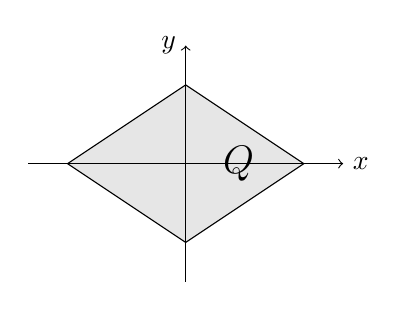
\begin{tikzpicture}[scale = 0.5]
  \coordinate (A) at (0, -2);
  \coordinate (B) at (3, 0);
  \coordinate (C) at (0, 2);
  \coordinate (D) at (-3, 0);

  \definecolor{lightGray}{HTML}{e6e6e6};
  \filldraw[fill = lightGray] (A) -- (B) -- (C) -- (D) -- cycle;


  \draw[->] (-4,0) -- (4,0) node[right] {$x$};
  \draw[->] (0,-3) -- (0,3) node[left] {$y$};

  \coordinate [label = {right: \Large $Q$}] (F) at (0.7, 0);
\end{tikzpicture}
\end{wrapfigure}

Нами доказана теорема:
\begin{theorem}
Пусть $\begin{cases} u_0(x)\in C^2(-l,l) \\ u_1(x) \in C^1(-l,l) \end{cases}$. Тогда ЗК имеет в $Q$\\[0.1em]
единственное решение $u(t,x)\in C^2(Q)$ -- классическое. Оно дается\\[0.1em] 
формулой Даламбера.
\end{theorem}

\imaginarySubsection{Корректность}
Корректность задачи для уравнения малых колебаний струны:
\begin{itemize}
\item нами проверены существование и единственность классического решения.
\item покажем непрерывность решения по входным данным $u_0$ и $u_1$.\\Берем две задачи:
\[ 
\begin{cases} 
  \overset{\text{\tiny{1}}}{u}_{tt}-a^2\overset{\text{\tiny{1}}}{u}_{xx} = 0, &(t,x)\in Q\\

  \overset{\text{\tiny{1}}}{u}\bigr|_{t=0} = \overset{\text{\tiny{1}}}{u}_0(x), &\abs*{x}<l\\ 
  
  \overset{\text{\tiny{1}}}{u}_t\bigr|_{t=0} = \overset{\text{\tiny{1}}}{u}_1(x), &\abs*{x}<l\end{cases} \qquad
\begin{cases} 
  \overset{\text{\tiny{2}}}{u}_{tt}-a^2\overset{\text{\tiny{2}}}{u}_{xx} = 0, &(t,x)\in Q\\

  \overset{\text{\tiny{2}}}{u}\bigr|_{t=0} = \overset{\text{\tiny{2}}}{u}_0(x), &\abs*{x}<l\\

  \overset{\text{\tiny{2}}}{u}_t\bigr|_{t=0} = \overset{\text{\tiny{2}}}{u}_1(x), &\abs*{x}<l
\end{cases}
\]
Пусть $\abs*{\overset{\text{\tiny{1}}}{u}_0 - \overset{\text{\tiny{2}}}{u}_0}<\delta_0,\ \abs*{\overset{\text{\tiny{1}}}{u}_1 - \overset{\text{\tiny{2}}}{u}_1}<\delta_1 \;\Forall x\colon \abs*{x}<l.$ \quad Введем 
$\begin{cases}
v_0 = \overset{\text{\tiny{1}}}{u}_0 - \overset{\text{\tiny{2}}}{u}_0 \\
v_1 = \overset{\text{\tiny{1}}}{u}_1 - \overset{\text{\tiny{2}}}{u}_1 \\
v = \overset{\text{\tiny{1}}}{u} - \overset{\text{\tiny{2}}}{u}
\end{cases}$\\
Тогда задача для $v:\ 
\begin{cases} 
v_{tt}-a^2v_{xx} = 0, \qquad (t,x) \in Q\\

\begin{aligned}
\eval{v}_{t=0}\; = v_0(x),\quad &\abs*{x}<l,\ \abs*{v_0}<\delta_0\\

\eval{v_t}_{t=0} = v_1(x),\quad &\abs*{x}<l,\ \abs*{v_1}<\delta_1
\end{aligned}

\end{cases}$
\vspace{0.2em}

Согласно формуле Даламбера,
$$\abs*{v(t,x)} = \abs*{\dfrac{v_0(x+at) + v_0(x-at)}{2} + \dfrac1{2a}\int\limits_{x-at}^{x+at}v_1(y)dy} \leq \delta_0 + \delta_1t \;\; \Forall (t,x) \in Q$$

\begin{itemize}
\item[--] Если $l$ конечно, то $t\le \dfrac{l}{a}$ из вида четырёхугольника $Q$. Устремляя $\delta_0,\, \delta_1 \to 0$, \\
получим $\abs*{v}\to 0$.
\item[--] Если $l=\infty$: в любой конечной полосе $t\le T< \infty$ требуемое верно. \\
Так заметаем всю плоскость.


\end{itemize}
\end{itemize}

\end{document}